C9/C24 ranks first with $A=396$~m$^2$, $H=0.04874$~h and nominal $V=5551.333$~m$^3$. Its rule reduces the modeled heights of C9 and C24 from 12 and 9~m to 9 and 6.75~m. C9/C15 offers $351$~m$^2$ with a smaller nominal proxy of $3127.755$~m$^3$, while C9/C13 offers $333$~m$^2$ at $2975.156$~m$^3$. These three are also on the full-universe area--volume front. The values give an architect reasons to inspect different benefit--cost positions; they do not establish actual removal quantities, legal eligibility or construction feasibility.

The score is not an area-only ranking. For example, C15/C24 ranks fourth with $243$~m$^2$ of area reduction and $0.05367$~h mean gain, while C9/C13 ranks sixth with $333$~m$^2$ and $0.03028$~h. C12/C24 ranks seventh despite a smaller area benefit of $198$~m$^2$, because its mean gain is $0.06228$~h. This is a consequence of the declared normalization and weights rather than an error to be corrected by substituting an area ranking. Figure~\ref{fig:choice} shows the complementary $A/V$ view across all 630 candidates.

\begin{figure}[tbp]\centering
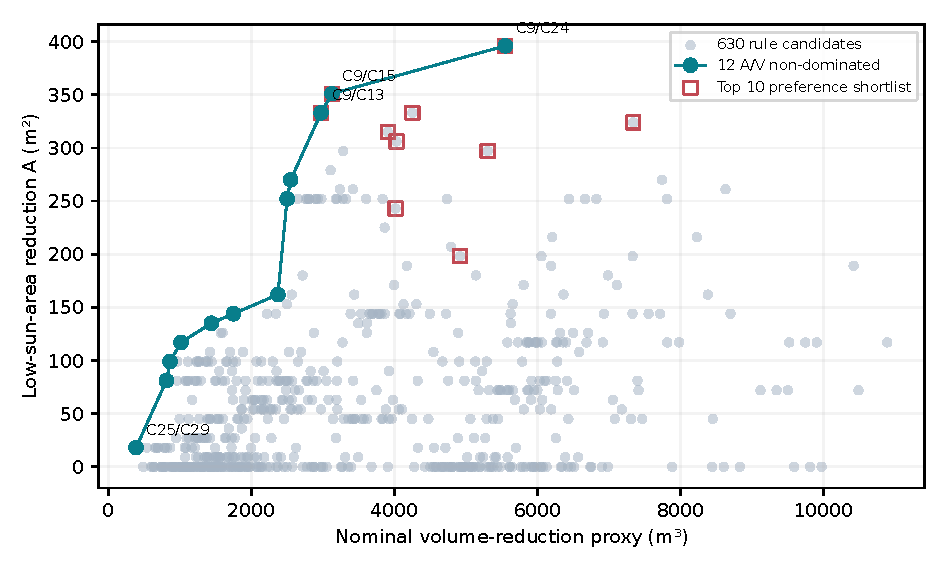
\includegraphics[width=\textwidth]{figures/candidate_tradeoff.pdf}
\Description{Full candidate universe plotted by nominal volume proxy and low-sun-area reduction, with the top ten and nondominated candidates highlighted. The plot displays the finite modeled choice set, not site geometry.}
\caption{The complete area--nominal-volume choice set, recomputed from archived candidate aggregates. The top ten follow the four-term score; the Pareto front uses only $A$ and $V$. This aggregate plot contains no site coordinates or newly simulated observations.}
\label{fig:choice}
\end{figure}

All twelve nondominated candidates have nonzero area benefit. Three also appear in the top ten, giving nineteen distinct score-selected or Pareto candidates. Adding historical pairs C6/C33 and C13/C24 and reference pairs C3/C19 and C26/C35 yields the curated 23. The reference pairs are interventions used for comparison; they are not the unchanged baseline scene. This review pool covers 23/630, or approximately 3.65\%, of the rule universe. The fraction describes selection effort, not verified global recall or a measured saving in the whole design process.

Every top-ten rule has an archived Honeybee result. Area reduction agrees exactly for nine of the ten; C9/C27 has $324$~m$^2$ in screening and $333$~m$^2$ in the archived rule review. Design-translation evidence is much narrower: only C9/C24 and C9/C15 have checked contained corrections, while C9/C13 reuses an already-contained result. The other seven rows have no archived translated-design verification. In particular, the first-ranked rule's $396$~m$^2$ result must not be mistaken for the corrected translation's $351$~m$^2$. A reviewed rule is evidence for further assessment, not a completed design.
